\begin{enunciado}{2}
    Show that for the learning model of positive rectangles (aligned horizontally or vertically), $m_{\hipotset}(4) = 2^4$ and $m_{\hipotset}(5) < 2^5$. Hence, give a bound for $m_{\hipotset}(N)$.
\end{enunciado}

A figura abaixo mostra como podemos separar 4 pontos utilizando retângulos positivos alinhados horizontalmente ou verticalmente.

\begin{figure}[h]
	\centering
	\begin{minipage}{0.46\textwidth}
		\centering
		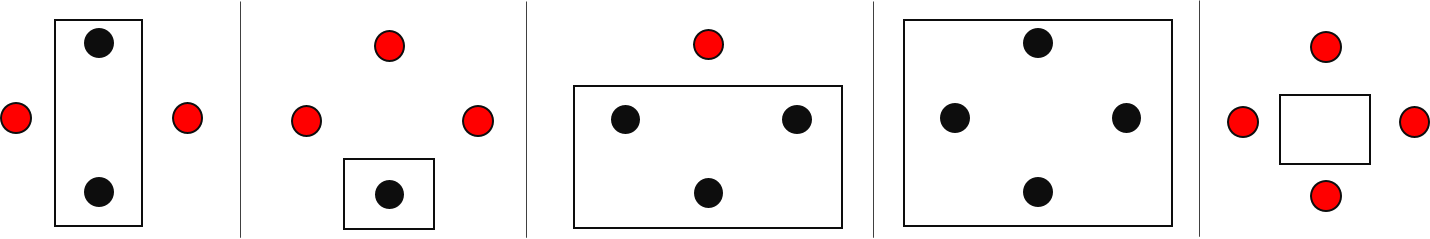
\includegraphics[width=\textwidth]{images/2-2-dvc4.png}
		\caption{Arranjo de 4 pontos que podem ser estraçalhados}
	\end{minipage}
\end{figure}

Logo, como queríamos demonstrar, $m_{\hipotset}(4) = 2^4$.


Precisamos mostrar, também, que $m_{\hipotset}(5) < 2^5$.
Portanto, dados 5 pontos, uma combinação possível que pode ser estraçalhada deve nos permitir selecionar todos os 5 pontos
e, também, selecionar 4 pontos sem o quinto.

\begin{figure}[h]
	\centering
	\begin{minipage}{0.45\textwidth}
		\centering
		
\includegraphics[width=\textwidth]{images/2-2-dvc5.png}
		\caption{Arranjo de 5 pontos que não podem ser estraçalhados}
	\end{minipage}
\end{figure}

Logo, vê-se que o retângulo que nos permite selecionar todos os 5 pontos é definido por apenas 4 pontos
- um para cada aresta. Assim, é evidente que o quinto ponto deve situar-se quer por uma aresta ou no interior do
retângulo. Isso nos impede de selecionar 4 pontos sem o quinto, o que prova que $m_{\hipotset}(5) < 2^5$.\\

Agora, vamos atribuir um limite para $m_{\hipotset}(N)$, como solicitado no enunciado.

Pela definição do breakpoint, se nenhum conjunto de dados de tamanho $k$ pode ser estraçalhado por ${\hipotset}$, então $k$ é dito
ser um breakpoint de ${\hipotset}$. Como demonstrado acima, para o problema dos retângulos positivos alinhados 
horizontalmente ou verticalmente, temos que $k = 5$.

Além disso, se $m(k)<2^k$ para algum $k$, então a função de crescimento $m_{\hipotset}(N) \le N^{k-1} + 1$.
Logo, $m_{\hipotset}(N) \le N^4+1$.